


\tikzset{every picture/.style={line width=0.75pt}} %set default line width to 0.75pt        

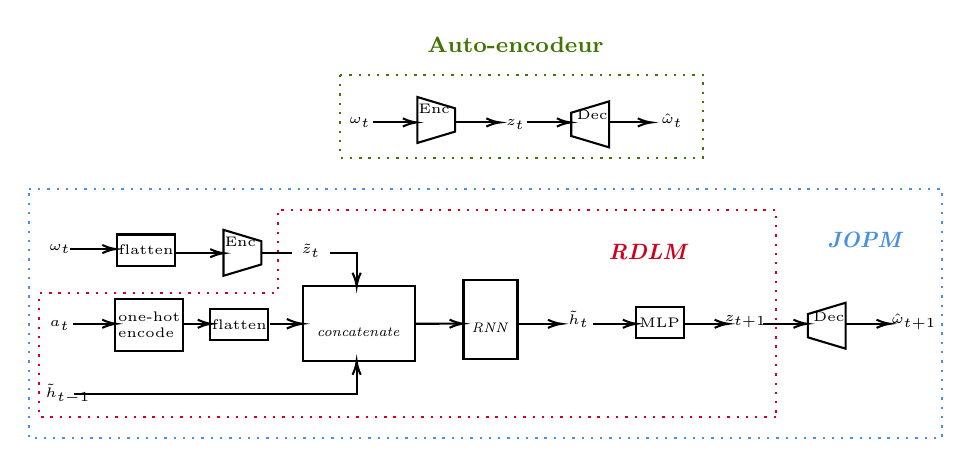
\begin{tikzpicture}[x=0.75pt,y=0.75pt,yscale=-1,xscale=1]
    %uncomment if require: \path (0,2102); %set diagram left start at 0, and has height of 2102

    %Straight Lines [id:da7905055997256106] 
    \draw    (53.06,1235.47) -- (73.06,1235.47) ;
    \draw [shift={(75.06,1235.47)}, rotate = 180] [color={rgb, 255:red, 0; green, 0; blue, 0 }  ][line width=0.75]    (6.56,-1.97) .. controls (4.17,-0.84) and (1.99,-0.18) .. (0,0) .. controls (1.99,0.18) and (4.17,0.84) .. (6.56,1.97)   ;
    %Straight Lines [id:da5451220917566785] 
    \draw    (54.23,1271.47) -- (73.06,1271.47) ;
    \draw [shift={(75.06,1271.47)}, rotate = 180] [color={rgb, 255:red, 0; green, 0; blue, 0 }  ][line width=0.75]    (6.56,-1.97) .. controls (4.17,-0.84) and (1.99,-0.18) .. (0,0) .. controls (1.99,0.18) and (4.17,0.84) .. (6.56,1.97)   ;
    %Straight Lines [id:da4433866589105997] 
    \draw    (55.06,1305.47) -- (191.06,1305.47) -- (191.06,1291.47) ;
    \draw [shift={(191.06,1289.47)}, rotate = 90] [color={rgb, 255:red, 0; green, 0; blue, 0 }  ][line width=0.75]    (6.56,-1.97) .. controls (4.17,-0.84) and (1.99,-0.18) .. (0,0) .. controls (1.99,0.18) and (4.17,0.84) .. (6.56,1.97)   ;
    %Straight Lines [id:da9772153219599438] 
    \draw    (107.06,1271.47) -- (119.06,1271.47) ;
    \draw [shift={(121.06,1271.47)}, rotate = 180] [color={rgb, 255:red, 0; green, 0; blue, 0 }  ][line width=0.75]    (6.56,-1.97) .. controls (4.17,-0.84) and (1.99,-0.18) .. (0,0) .. controls (1.99,0.18) and (4.17,0.84) .. (6.56,1.97)   ;
    %Straight Lines [id:da08798558878605356] 
    \draw    (149.44,1271.47) -- (163.06,1271.47) ;
    \draw [shift={(165.06,1271.47)}, rotate = 180] [color={rgb, 255:red, 0; green, 0; blue, 0 }  ][line width=0.75]    (7.65,-2.3) .. controls (4.86,-0.97) and (2.31,-0.21) .. (0,0) .. controls (2.31,0.21) and (4.86,0.98) .. (7.65,2.3)   ;
    %Straight Lines [id:da5508296944602415] 
    \draw    (103.06,1237.47) -- (125.06,1237.47) ;
    \draw [shift={(127.06,1237.47)}, rotate = 180] [color={rgb, 255:red, 0; green, 0; blue, 0 }  ][line width=0.75]    (6.56,-1.97) .. controls (4.17,-0.84) and (1.99,-0.18) .. (0,0) .. controls (1.99,0.18) and (4.17,0.84) .. (6.56,1.97)   ;
    %Shape: Trapezoid [id:dp14410290094148615] 
    \draw   (126.9,1226.21) -- (145.13,1231.68) -- (145.13,1242.88) -- (126.9,1248.35) -- cycle ;
    %Straight Lines [id:da384443735490001] 
    \draw    (145.06,1237.47) -- (191.06,1237.47) -- (191.06,1251.47) ;
    \draw [shift={(191.06,1253.47)}, rotate = 270] [color={rgb, 255:red, 0; green, 0; blue, 0 }  ][line width=0.75]    (6.56,-1.97) .. controls (4.17,-0.84) and (1.99,-0.18) .. (0,0) .. controls (1.99,0.18) and (4.17,0.84) .. (6.56,1.97)   ;
    %Straight Lines [id:da5196284966358902] 
    \draw    (219.06,1271.47) -- (240.39,1271.41) ;
    \draw [shift={(242.39,1271.41)}, rotate = 179.85] [color={rgb, 255:red, 0; green, 0; blue, 0 }  ][line width=0.75]    (6.56,-1.97) .. controls (4.17,-0.84) and (1.99,-0.18) .. (0,0) .. controls (1.99,0.18) and (4.17,0.84) .. (6.56,1.97)   ;
    %Straight Lines [id:da2885650017773205] 
    \draw    (268.95,1271.5) -- (287.78,1271.5) ;
    \draw [shift={(289.78,1271.5)}, rotate = 180] [color={rgb, 255:red, 0; green, 0; blue, 0 }  ][line width=0.75]    (6.56,-1.97) .. controls (4.17,-0.84) and (1.99,-0.18) .. (0,0) .. controls (1.99,0.18) and (4.17,0.84) .. (6.56,1.97)   ;
    %Straight Lines [id:da1683388835537969] 
    \draw    (305.06,1271.47) -- (323.89,1271.47) ;
    \draw [shift={(325.89,1271.47)}, rotate = 180] [color={rgb, 255:red, 0; green, 0; blue, 0 }  ][line width=0.75]    (6.56,-1.97) .. controls (4.17,-0.84) and (1.99,-0.18) .. (0,0) .. controls (1.99,0.18) and (4.17,0.84) .. (6.56,1.97)   ;
    %Straight Lines [id:da18138221495614015] 
    \draw    (349.06,1271.47) -- (356.46,1271.47) -- (368.1,1271.47) ;
    \draw [shift={(370.1,1271.47)}, rotate = 180] [color={rgb, 255:red, 0; green, 0; blue, 0 }  ][line width=0.75]    (6.56,-1.97) .. controls (4.17,-0.84) and (1.99,-0.18) .. (0,0) .. controls (1.99,0.18) and (4.17,0.84) .. (6.56,1.97)   ;
    %Shape: Trapezoid [id:dp15428640042958097] 
    \draw   (426.67,1283.47) -- (408.44,1278) -- (408.44,1266.79) -- (426.67,1261.32) -- cycle ;
    %Straight Lines [id:da8308982689158874] 
    \draw    (387.06,1271.47) -- (406.1,1271.47) ;
    \draw [shift={(408.1,1271.47)}, rotate = 180] [color={rgb, 255:red, 0; green, 0; blue, 0 }  ][line width=0.75]    (6.56,-1.97) .. controls (4.17,-0.84) and (1.99,-0.18) .. (0,0) .. controls (1.99,0.18) and (4.17,0.84) .. (6.56,1.97)   ;
    %Straight Lines [id:da854779381814783] 
    \draw    (427.06,1271.47) -- (446.1,1271.47) ;
    \draw [shift={(448.1,1271.47)}, rotate = 180] [color={rgb, 255:red, 0; green, 0; blue, 0 }  ][line width=0.75]    (6.56,-1.97) .. controls (4.17,-0.84) and (1.99,-0.18) .. (0,0) .. controls (1.99,0.18) and (4.17,0.84) .. (6.56,1.97)   ;
    %Shape: Trapezoid [id:dp12236333694521873] 
    \draw   (220.29,1162.21) -- (238.52,1167.68) -- (238.52,1178.88) -- (220.29,1184.35) -- cycle ;
    %Shape: Trapezoid [id:dp4232724503855386] 
    \draw   (312.67,1186.47) -- (294.44,1181) -- (294.44,1169.79) -- (312.67,1164.32) -- cycle ;
    %Straight Lines [id:da0811328179216142] 
    \draw    (313.06,1174.47) -- (331.06,1174.47) ;
    \draw [shift={(333.06,1174.47)}, rotate = 180] [color={rgb, 255:red, 0; green, 0; blue, 0 }  ][line width=0.75]    (6.56,-1.97) .. controls (4.17,-0.84) and (1.99,-0.18) .. (0,0) .. controls (1.99,0.18) and (4.17,0.84) .. (6.56,1.97)   ;
    %Straight Lines [id:da33212985731507805] 
    \draw    (199.06,1174.47) -- (217.89,1174.47) ;
    \draw [shift={(219.89,1174.47)}, rotate = 180] [color={rgb, 255:red, 0; green, 0; blue, 0 }  ][line width=0.75]    (6.56,-1.97) .. controls (4.17,-0.84) and (1.99,-0.18) .. (0,0) .. controls (1.99,0.18) and (4.17,0.84) .. (6.56,1.97)   ;
    %Straight Lines [id:da7950301814204398] 
    \draw    (239.06,1174.47) -- (258.1,1174.47) ;
    \draw [shift={(260.1,1174.47)}, rotate = 180] [color={rgb, 255:red, 0; green, 0; blue, 0 }  ][line width=0.75]    (6.56,-1.97) .. controls (4.17,-0.84) and (1.99,-0.18) .. (0,0) .. controls (1.99,0.18) and (4.17,0.84) .. (6.56,1.97)   ;
    %Straight Lines [id:da8317125190119203] 
    \draw    (273.06,1174.47) -- (292.1,1174.47) ;
    \draw [shift={(294.1,1174.47)}, rotate = 180] [color={rgb, 255:red, 0; green, 0; blue, 0 }  ][line width=0.75]    (6.56,-1.97) .. controls (4.17,-0.84) and (1.99,-0.18) .. (0,0) .. controls (1.99,0.18) and (4.17,0.84) .. (6.56,1.97)   ;
    %Shape: Polygon [id:ds33250073085001886] 
    \draw  [color={rgb, 255:red, 208; green, 2; blue, 27 }  ,draw opacity=1 ][dash pattern={on 0.84pt off 2.51pt}] (393.06,1316.47) -- (38.06,1316.47) -- (38.06,1256.47) -- (153.06,1256.47) -- (153.06,1216.47) -- (393.06,1216.47) -- cycle ;
    %Shape: Rectangle [id:dp3415456817493894] 
    \draw  [color={rgb, 255:red, 74; green, 144; blue, 226 }  ,draw opacity=1 ][dash pattern={on 0.84pt off 2.51pt}] (33.06,1206.47) -- (473.06,1206.47) -- (473.06,1326.47) -- (33.06,1326.47) -- cycle ;
    %Shape: Rectangle [id:dp9296059531842202] 
    \draw  [color={rgb, 255:red, 65; green, 117; blue, 5 }  ,draw opacity=1 ][dash pattern={on 0.84pt off 2.51pt}] (183.06,1151.47) -- (358.06,1151.47) -- (358.06,1191.47) -- (183.06,1191.47) -- cycle ;


    % Text Node
    \draw (332.06,1236.97) node  [color={rgb, 255:red, 208; green, 2; blue, 27 }  ,opacity=1 ] [align=left] {\footnotesize \textbf{\textit{RDLM}}};
    % Text Node
    \draw (436.56,1230.97) node  [color={rgb, 255:red, 74; green, 144; blue, 226 }  ,opacity=1 ] [align=left] {\footnotesize \textbf{\textit{JOPM}}};
    % Text Node
    \draw (267.56,1136.97) node  [color={rgb, 255:red, 65; green, 117; blue, 5 }  ,opacity=1 ] [align=left] {{\footnotesize \textbf{Auto-encodeur}}};
    % Text Node
    \draw (192.56,1174.47) node  [font=\tiny] [align=left] {$\displaystyle \omega _{t}$};
    % Text Node
    \draw (343.06,1173.47) node  [font=\tiny] [align=left] {$\displaystyle \hat{\omega }_{t}$};
    % Text Node
    \draw (304.56,1170.97) node   [align=left] {{\tiny Dec}};
    % Text Node
    \draw (228.44,1167.97) node   [align=left] {{\tiny Enc}};
    % Text Node
    \draw (267.56,1175.47) node  [font=\tiny] [align=left] {$\displaystyle z_{t}$};
    % Text Node
    \draw (459.6,1270.47) node  [font=\tiny] [align=left] {$\displaystyle \hat{\omega }_{t+1}$};
    % Text Node
    \draw (418.56,1267.97) node   [align=left] {{\tiny Dec}};
    % Text Node
    \draw (378.56,1270.47) node  [font=\tiny] [align=left] {$\displaystyle z_{t+1}$};
    % Text Node
    \draw (135.06,1231.97) node   [align=left] {{\tiny Enc}};
    % Text Node
    \draw (298.06,1269.47) node  [font=\tiny] [align=left] {$\displaystyle \tilde{h}_{t}$};
    % Text Node
    \draw    (242.54,1250.47) -- (268.54,1250.47) -- (268.54,1288.47) -- (242.54,1288.47) -- cycle  ;
    \draw (255.54,1269.47) node  [font=\tiny] [align=left] {\begin{minipage}[lt]{14.99pt}\setlength\topsep{0pt}
            \begin{center}
                \phantom{X}\\\textit{RNN}
            \end{center}

        \end{minipage}};
    % Text Node
    \draw  [color={rgb, 255:red, 255; green, 255; blue, 255 }  ,draw opacity=1 ][fill={rgb, 255:red, 255; green, 255; blue, 255 }  ,fill opacity=1 ]  (160.56,1227.47) -- (177.56,1227.47) -- (177.56,1245.47) -- (160.56,1245.47) -- cycle  ;
    \draw (169.06,1236.47) node  [font=\tiny] [align=left] {$\displaystyle \tilde{z}_{t}$};
    % Text Node
    \draw    (165.06,1253.47) -- (219.06,1253.47) -- (219.06,1289.47) -- (165.06,1289.47) -- cycle  ;
    \draw (192.06,1271.47) node  [font=\tiny] [align=left] {\begin{minipage}[lt]{34pt}\setlength\topsep{0pt}
            \begin{center}
                \phantom{X}\\\textit{concatenate}
            \end{center}

        \end{minipage}};
    % Text Node
    \draw    (120.56,1264.47) -- (148.56,1264.47) -- (148.56,1279.47) -- (120.56,1279.47) -- cycle  ;
    \draw (134.56,1271.97) node  [font=\tiny] [align=left] {flatten};
    % Text Node
    \draw (52.06,1305.47) node  [font=\tiny] [align=left] {$\displaystyle \tilde{h}_{t-1}$};
    % Text Node
    \draw (48.06,1272.47) node  [font=\tiny] [align=left] {$\displaystyle a_{t}$};
    % Text Node
    \draw (48.06,1235.47) node  [font=\tiny] [align=left] {$\displaystyle \omega _{t}$};
    % Text Node
    \draw    (325.56,1263.47) -- (348.56,1263.47) -- (348.56,1278.47) -- (325.56,1278.47) -- cycle  ;
    \draw (337.06,1270.97) node  [font=\tiny] [align=left] {MLP};
    % Text Node
    \draw    (74.56,1259.47) -- (107.56,1259.47) -- (107.56,1284.47) -- (74.56,1284.47) -- cycle  ;
    \draw (91.06,1271.97) node  [font=\tiny] [align=left] {one-hot\\encode};
    % Text Node
    \draw    (75.56,1228.47) -- (103.56,1228.47) -- (103.56,1243.47) -- (75.56,1243.47) -- cycle  ;
    \draw (89.56,1235.97) node  [font=\tiny] [align=left] {flatten};


\end{tikzpicture}